\subsection{Test of CAN, queues}
In order to test CAN and queues, a task was written. The purpose of the task was to receive a CAN-message if any available from the queue and send the ID and data from the CAN message to a PC using UART.
The task used can be seen in code \ref{code:test_can_uart_task}.


\begin{lstlisting}[language = c, caption = Task used to test CAN, label=code:test_can_uart_task]
CAN_frame frame;
if(QueueReceive(&Queue_CAN_Rx, &frame)) {
	char ch;
	/* ID out uart0 */
	for(int i = 3; i >=0; i--){
		ch = ((frame.id >> i*8) & 0x000000FF);
		QueueSend(&Queue_Uart0_Tx,&ch);
	}
	/* ID end*/

	/* MSG out uart0 */
	for(int i = (frame.dlc-1); i >=0; i--){
		ch = ((frame.msg >> i*8) & 0x00000000000000FF);
		QueueSend(&Queue_Uart0_Tx,&ch);
	}
	/* MSG end */

	/* End of line */
	ch = '\r';
	QueueSend(&Queue_Uart0_Tx,&ch);
	ch = '\n';
	QueueSend(&Queue_Uart0_Tx,&ch);
}
\end{lstlisting}
The command used to send CAN-messages can be seen in code \ref{code:bash_send_can}.

\begin{lstlisting}[language = bash, caption = Task used to test CAN, label=code:bash_send_can]
while true; do sleep 1; print $(date); cansend can0  1DEADBEF#FEDCBA9876543210; done
\end{lstlisting}
The command sends a CAN-message using a connected PEAK-CAN adapter. It sends a message each second and prints out the date to make it clear when it is sending a message.\\ \textit{1deadbef} is the 29 bit ID and \textit{fedcba9876543210} is the 64 bit data. \\


The command used to show the received HEX values can be seen in code \ref{code:xxd}

\begin{lstlisting}[language = bash, caption = Command used to get UART messages, label=code:xxd]
cat /dev/ttyUSB0 | xxd -c 14 
\end{lstlisting}
Cat reads from /dev/ttyUSB0 and pipes its output to xxd where it is shown in HEX.\\ -c is number of columns which is 14 due to 4 ID bytes, 8 data bytes and 2 as newline.\\

The result can be seen in figure \ref{fig:can_recv_output}.
\begin{figure}[H]
    \center
    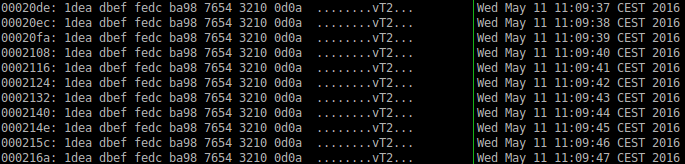
\includegraphics[width=1\textwidth]{graphics/xdd_can_test.png}
  \label{fig:boat1}
  \caption{Left shows output from command \ref{code:xxd} and right shows command \ref{code:bash_send_can}}
\end{figure}
It can be seen that the received ID and data is \textit{1deadbef} and \textit{fedcba9876543210} respectively.\\
\textit{0d0a} is \textbackslash r and \textbackslash n respectively.


\subsection{Test of RTCS timing}
In order to test the timing of the scheduler, a led\_task was written. The task can be seen in code \ref{code:test_scheduler}
\begin{lstlisting}[language = c, caption = RTCS task used in timing test, label=code:test_scheduler]
void is_alive_task(uint8_t my_state){

	// Write to UART0
	UDR0 = my_state+'0';

	switch(my_state){
	case 0:
		INT_LED_ON_GREEN;
		INT_LED_OFF_RED;
		INT_LED_OFF_BLUE;
	    set_state( 1 );
		break;
	case 1:
		INT_LED_OFF_GREEN;
		INT_LED_ON_RED;
		INT_LED_OFF_BLUE;
	    set_state( 2 );
		break;
	case 2:
		INT_LED_OFF_GREEN;
		INT_LED_OFF_RED;
		INT_LED_ON_BLUE;

		// Set next state
	    set_state( 0 );
		break;
	}
	// Wait one second
	wait( 1000 );
}
\end{lstlisting}

The test was done by writing the current state of the task to UART0.\\ A python script were made that measures the time between each character received. The script can be seen in code \ref{code:test_rtcs_python}.
\begin{lstlisting}[language = python, caption = Python code used to measure time between received byte, label=code:test_rtcs_python]
#!/usr/bin/python
import serial
import time

ser = serial.Serial( port='/dev/ttyUSB0', baudrate=57600 )

t = time.time()
while True:
    for char in ser.read(1):
        print time.time() - t, ","
        t = time.time()

ser.close()
\end{lstlisting}
The output of the script were redirected to a file. After receiving 700 bytes the standard deviation and mean was calculated using matlab.
The mean is 1.0089 sec with a standard deviation of 0.0042 sec.

Part of the variance is caused by the inaccuracy of the timing on the PC running the python code. If a more accurate measure was needed, a scope could be attached to the $\mu$C's GPIO. Each time the scheduler enters the task the GPIO should be set high, and when it exists the GPIO should be set low. The scopes at SDU is capable of telling the variance of the off signal. \\
It can be concluded that the scheduler performs well.